\documentclass[]{article}
\usepackage{lmodern}
\usepackage{amssymb,amsmath}
\usepackage{ifxetex,ifluatex}
\usepackage{fixltx2e} % provides \textsubscript
\ifnum 0\ifxetex 1\fi\ifluatex 1\fi=0 % if pdftex
  \usepackage[T1]{fontenc}
  \usepackage[utf8]{inputenc}
\else % if luatex or xelatex
  \ifxetex
    \usepackage{mathspec}
  \else
    \usepackage{fontspec}
  \fi
  \defaultfontfeatures{Ligatures=TeX,Scale=MatchLowercase}
\fi
% use upquote if available, for straight quotes in verbatim environments
\IfFileExists{upquote.sty}{\usepackage{upquote}}{}
% use microtype if available
\IfFileExists{microtype.sty}{%
\usepackage{microtype}
\UseMicrotypeSet[protrusion]{basicmath} % disable protrusion for tt fonts
}{}
\usepackage[margin=1in]{geometry}
\usepackage{hyperref}
\hypersetup{unicode=true,
            pdfborder={0 0 0},
            breaklinks=true}
\urlstyle{same}  % don't use monospace font for urls
\usepackage{graphicx,grffile}
\makeatletter
\def\maxwidth{\ifdim\Gin@nat@width>\linewidth\linewidth\else\Gin@nat@width\fi}
\def\maxheight{\ifdim\Gin@nat@height>\textheight\textheight\else\Gin@nat@height\fi}
\makeatother
% Scale images if necessary, so that they will not overflow the page
% margins by default, and it is still possible to overwrite the defaults
% using explicit options in \includegraphics[width, height, ...]{}
\setkeys{Gin}{width=\maxwidth,height=\maxheight,keepaspectratio}
\IfFileExists{parskip.sty}{%
\usepackage{parskip}
}{% else
\setlength{\parindent}{0pt}
\setlength{\parskip}{6pt plus 2pt minus 1pt}
}
\setlength{\emergencystretch}{3em}  % prevent overfull lines
\providecommand{\tightlist}{%
  \setlength{\itemsep}{0pt}\setlength{\parskip}{0pt}}
\setcounter{secnumdepth}{0}
% Redefines (sub)paragraphs to behave more like sections
\ifx\paragraph\undefined\else
\let\oldparagraph\paragraph
\renewcommand{\paragraph}[1]{\oldparagraph{#1}\mbox{}}
\fi
\ifx\subparagraph\undefined\else
\let\oldsubparagraph\subparagraph
\renewcommand{\subparagraph}[1]{\oldsubparagraph{#1}\mbox{}}
\fi

%%% Use protect on footnotes to avoid problems with footnotes in titles
\let\rmarkdownfootnote\footnote%
\def\footnote{\protect\rmarkdownfootnote}

%%% Change title format to be more compact
\usepackage{titling}

% Create subtitle command for use in maketitle
\newcommand{\subtitle}[1]{
  \posttitle{
    \begin{center}\large#1\end{center}
    }
}

\setlength{\droptitle}{-2em}

  \title{}
    \pretitle{\vspace{\droptitle}}
  \posttitle{}
    \author{}
    \preauthor{}\postauthor{}
    \date{}
    \predate{}\postdate{}
  

\begin{document}

\chapter{Methods}\label{ch:methods}

\section{Making social care data available for linkage}\label{sec:linkage}

Describe method of matching SCS to Population Spine

\section{Creating a linked health and social care dataset}\label{sec:make-dataset}

\FloatBarrier

\subsection{Setting and cohort}\label{subsec:setting-cohort}

Scotland has a population of around 5.4 million people. Health care has
been delivered via 14 territorial health boards whilst social care falls
withing the remit of the 32 local authorities. Since 2016, health and
social care services have been integrated and 31 Integrated Joint Boards
(IJBs) have been created.

The cohort included all individuals in Scotland born before 31st March
1951 and alive during the study period 1st April 2011 to 31st March
2016. This identified all those over the age of 65 (and those turning 65
during the study period). Data for the cohort was extracted from the
research population spine held by NRS with CHI numbers allowing linkage
to other datasets.

\begin{landscape}
\begin{figure}
  \centering
    \caption{Data linkage diagram}
    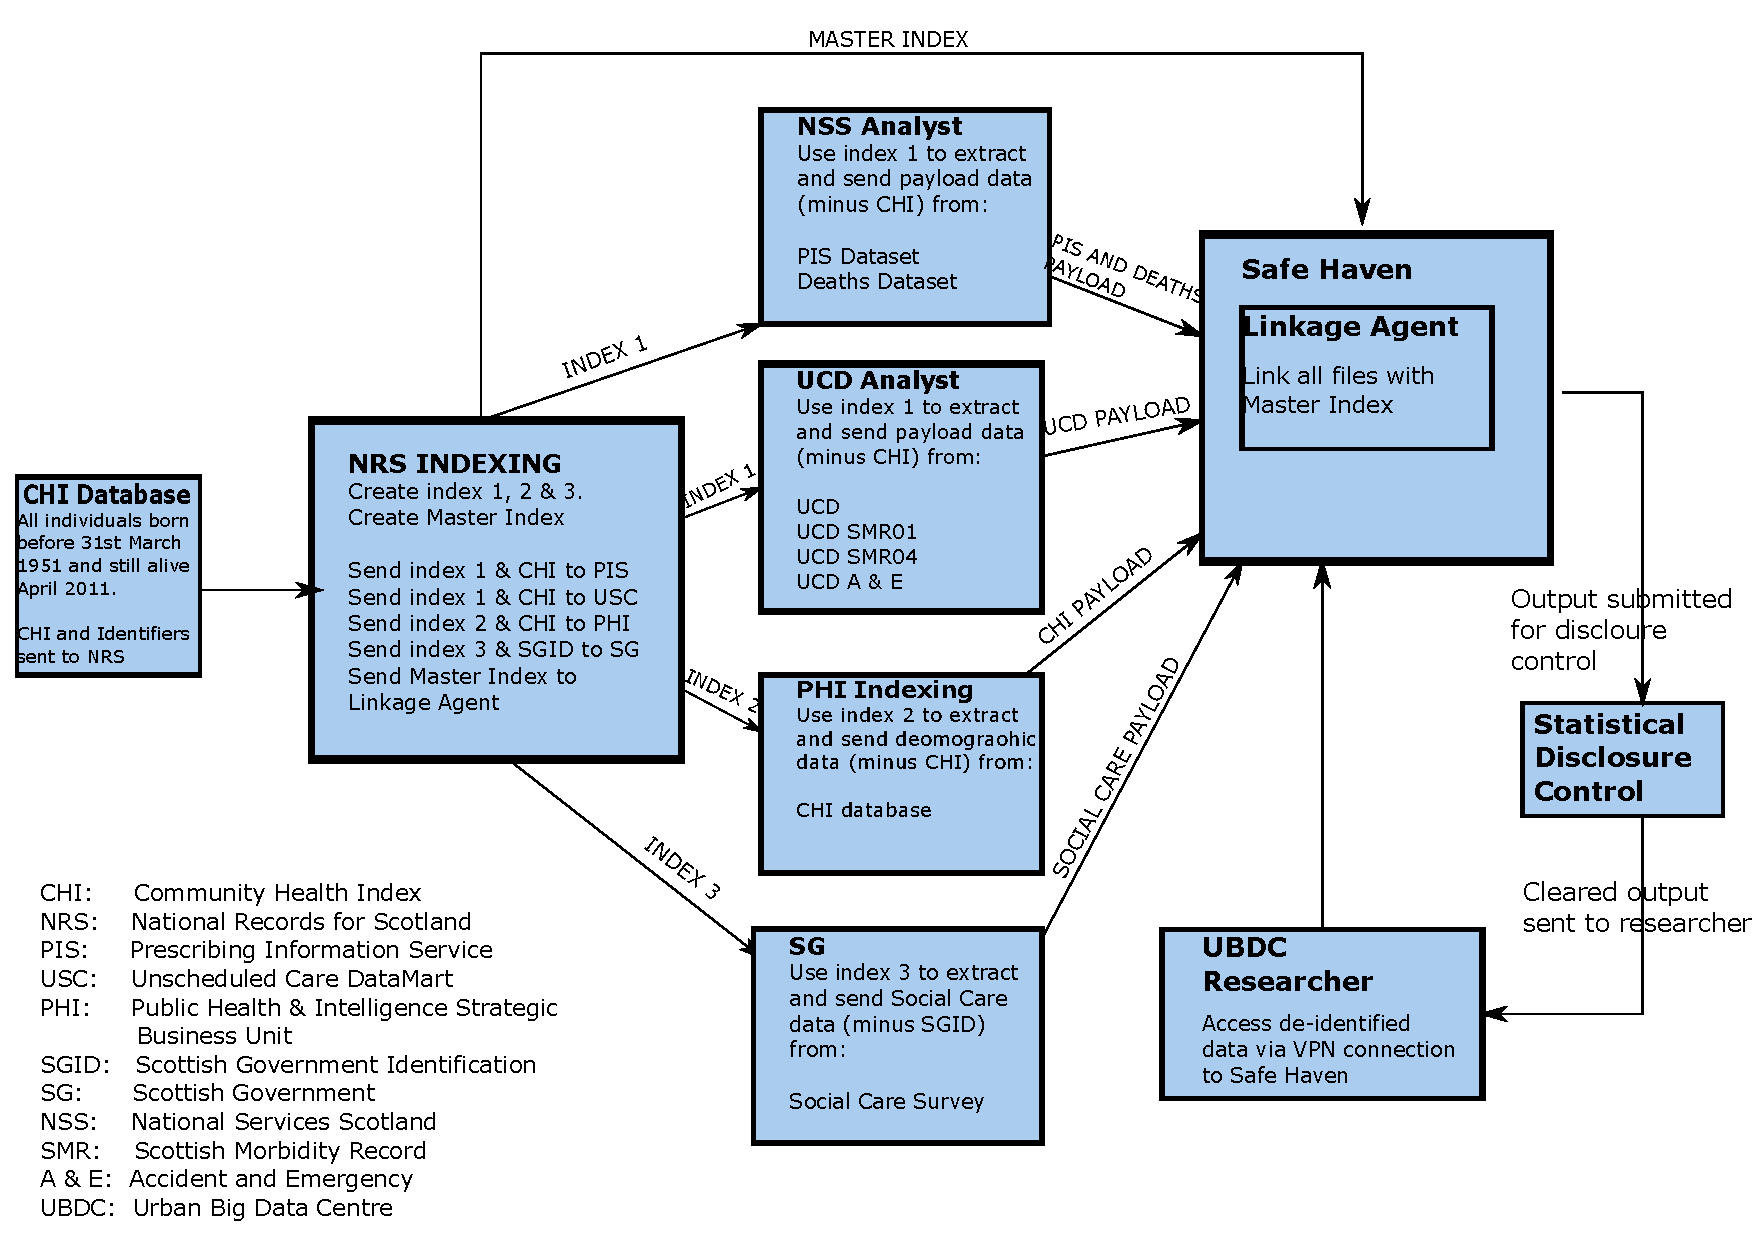
\includegraphics{data/produced_data/linkage-diagram/linkage-diagram.pdf}
    \label{fig:methods-linkage}
\end{figure}
\end{landscape}

As figure \ref{fig:methods-linkage} shows, linkage keys from the
extracted cohort were sent by an eDRIS coordinator to various health and
social care data sources for extraction of information relating to any
of these indivudals in the target data source. Specific variables
requested, the time period they were requested over, and cleaning and
wrangling of these data sources is described in the following section.

\textbf{Figure needs tidied up and should show datasets in same order as
following subsections}

The aim of cleaning and wrangling was to create one row of data for each
indivudal for each financial year (1st April - 31st March) of the study
period. This format is based on the principals of tidy data
{[}@RN553{]}. Financial years were chosen as the time period of interest
because the social care survey reports home care usage in a census week
which is usually at the end of March. As each raw data file provided was
in differing formats, this required differing approaches and relied
heavily on data manipulation software packages \texttt{tidyr} v0.7.2
{[}@RN524{]}, \texttt{dplyr} v0.7.4 {[}@RN283{]}, \texttt{lubridate}
v1.6.0 {[}@RN522{]}, \texttt{stringr} v1.2.0 {[}@RN554{]}, and
\texttt{forcats} v0.2.0 {[}@RN521{]} in the R language and environment
for statistical computing version 3.4.0 {[}@RN295{]} via the Integrated
Development Environment RStudio v1.0.143 {[}@RN498{]}.

\FloatBarrier

\subsection{Demographic, geographic, and deaths information}\label{subsubsec:nrs-summs}

\begin{table}[h]
\centering
\caption{Demographic file data}
\label{tab:demos}
\resizebox{\textwidth}{!}{%
\begin{tabular}{@{}lll@{}}
\toprule
Number of rows & Number of individuals & Variables \\ \midrule
1,348,310 & 1,134,445 & \begin{tabular}[c]{@{}l@{}}Index, year/month of birth, year/month of death\\ Sex, Address start date, Address end date, Care home flag,\\ Previous Local Authority, Current Local Authority, \\ Current Health Board, SIMD decile\end{tabular} \\ \bottomrule
\end{tabular}%
}
\end{table}

Demographic information for all eligible indiviudals identified from the
population spine was extracted by the Public Health and Intelligence:
Strategic Business Unit at NSS. This was joined with a flag variable
indicating if an individual was resident in a care home (from
prescribing data) in a single file which was made available in the
national safe haven. SIMD decile was assigned as per the most recent
version of the area-based measure (2016). The number of observations,
individuals, and the differing variables in this raw demographic file
are shown in table \ref{tab:demos}.

As the table indicates some individuals had more than one row of
information indicating multiple addresses during the study period (and
thus potential multiple values for local, authority, health board, care
home flag, and SIMD decile). Financial year time intervals were created
for each financial year using the \texttt{lubridate} software package
{[}@RN522{]}. Dummy variables were then created indicating the age,
local authority of residence, health board of residence, and simd decile
during each financial year (with null values where not applicable). The
variables were then gathered to long format in order to reshape the data
to include one row of data per individual per financial year. Where and
individual had multiple addresses during one fininacial year, the most
recent value for local authority, health board, and SIMD decile was
used. This resulted in a dataframe of 7,775,410 observations pertaining
to 1,134,445 individuals.

\FloatBarrier

\subsection{Social Care Survey}\label{subsubsec:scs-summs}

Data from the Scottish Care Surveys 2010 - 2016 (including separate Home
Care Census and Self-Directed Support surveys for earlier years) were
extracted by a Scotish Government analyst and transferred to the
national safe haven in a single file. There were a number of variables
indicating the weekly hours of home care (if any) each indiviudal
received, whether they were provided by the local authority or and
independent orgainsation, and whether these hours indicated the
scheduled hours of home care or the actual number of hours delivered.
There is some discrepency between local authorities on which value
(scheduled, or actual) of home care is returned to the Scottish
Government for the SCS. Some authorities return scheduled only, others
actual hours only, and yet others return both values. The SCS reports
statistics based on the actual hours of home care delivered where
available and uses the scheduled value where it is not. This convention
was also used for the purposes of this thesis.

Many variables requested from the SCS had large amounts of missing data.
There were also coding issues with extra values present that had no
corresponding description in the provided metadata. Table
\ref{tab:scs-vars} lists the variables included and excluded after data
cleaning.

Assessment for duplicated rows indicated 4,357 individuals had more than
one row of data for some years of data. Inspection of these additional
rows indicated a change in value for some variables (e.g.~a flag
indicating use of community alarm services postive in one row and
negative in another, or different values for client group in multiple
rows). These additional rows amounted to 1.1\% of observations in the
SCS. Once joined to other datasets (as described in section
\ref{subsec:join-data}), all observations for the years of data where
there were duplicates were dropped from the dataset.

\begin{table}[]
\caption{Social Care Survey file data}
\label{tab:scs-vars}
\resizebox{\textwidth}{!}{%
\begin{tabular}{@{}lllll@{}}
\toprule
Number of rows & Number of individuals & Included variables & Derived variables & Dropped variables \\ \midrule
 &  & \begin{tabular}[c]{@{}l@{}}1. Index (ID)\\ 2. Living alone\\ 3. Community Alarm\\ 4. Other telecare\end{tabular} & \begin{tabular}[c]{@{}l@{}}1. Total weekly hours of homecare\\ 2. Home care hours group (e.g 1-5, 6-10 etc.)\\ 3. Alarm or Telecare flag\end{tabular} & \begin{tabular}[c]{@{}l@{}}1. Client Group\\ 2. Eligibility Category\\ 3. Housing Support\\ 4. Multi Staffing\\ 5. Scheduled Hours\\ 6. Actual Hours\end{tabular} \\ \bottomrule
\end{tabular}%
}
\end{table}

\FloatBarrier

\subsection{Prescribing Information Service}\label{subsec:pis-summs}

Community prescribing information for all individuals in the cohort were
extracted from the Prescribing Information System (PIS) by analysts from
ISD. For each quarter of the study period (Quarter 1 2010/11 to Quarter
4 2015/16) a list of medicines prescribed to each indiviudal was
extracted and transferred in one file to the national safe haven. This
file contained 134,377,877 observations of four variables: The financial
year and quarter, the BNF subsection code, The approved name of the
medicine, and a count of how many times the medicine was prescribed in
the quarter. Coding errors were found in 138,973 observations (wrong
number of digits in the BNF subsection or characters found in the count
variable) and these were dropped from analysis.

The count of medicines was based on the BNF classes included in a count
of polypharmacy by Guthrie et al {[}@RN274{]}. The additional material
provided online with this paper included a table of included drugs. This
table was ammended to remove BNF subsections 3.9.1, 3.9.2, and 13.9. The
latter section includes different forms of shampoos whilst the former 2
sections include preperations for coughs. These were not deemed
necessary to be included in overall counts. Two BNF subsections not
included in the Guthrie et al table were deemed important to include as
testing revealed large numbers of prescriptions included medicines from
these sections would have been omitted otherwise. These sections were
2.2.4 (Potassium sparing diuretics with other diuretics) and 2.2.8.
(Diuretics with potassium). In total, 198 medicines listed in the BNF
were not included and rows with these medicines were removed from the
PIS file. A full list of these medicines is shown in Appendix F. Table
\ref{tab:dropped-meds} shows the cleaning process.

\begin{table}[h]
\centering
\caption{Data cleaning of PIS file}
\label{tab:dropped-meds}
\begin{tabular}{@{}lll@{}}
\toprule
Reasons & Records dropped & Records remaining \\ \midrule
Initial data file & N/A & 134,377,877 \\
Coding errors & 138,973 & 134,238,904 \\
Did not appear in Guthrie et al (2012) table & 1,427,643 & 132,811,261 \\
BNF sections 3.9.1, 3.9.2, \& 13.9 & 645,900 & 132,165,361 \\ \bottomrule
\end{tabular}
\end{table}

A summary measure for each indiviudal was created counting the total
number of medicines prescribed in each financial year. To be eligible in
the count, a medicine had to be prescribed in at least 2 quarters of
each financial year. This meant one-off prescriptions, such as
antibiotics for a transient infection, were not included in the overall
count. An indiviudal could thus have a maximum of 6 observations, one
for each financial year. A second count was created totalling the number
of chapters of the BNF that each individual had medicines prescribed
from as a crude measure of body systems requiring medication. Table
\ref{tab:PIS-clean} shows the total observations and variables in the
cleaned PIS file.

\begin{table}[h]
\centering
\caption{Description of cleaned PIS file}
\label{tab:PIS-clean}
\begin{tabular}{@{}lll@{}}
\toprule
Number or rows & Number of individuals & Variables \\ \midrule
5,473,640 & 1,066,103 & \begin{tabular}[c]{@{}l@{}}1. Index (id)\\ 2. Financial Year\\ 3. Total medicines (n)\\ 4. Total chapters (n)\end{tabular} \\ \bottomrule
\end{tabular}
\end{table}

\FloatBarrier
\subsection{Unscheduled care measures}\label{subsec:usc-summs}

Which years of data (remember OOH from 2014 onwards only)

How was usc data wrangled? Which summary measures were chosen?

\subsection{Joining sources together}\label{subsec:join-data}

Dropping rows etc. Report final n observations and individuals.

Table of variables.

\section{Statistical methods}\label{sec:methods-stats}

\subsection{Descriptive statistics}\label{descr}

\subsection{Research question 1}\label{stats-rq1}

\subsection{Research question 2}\label{stats-rq2}


\end{document}
